% LTeX: language=it

\chapter{Architettura del compilatore}
\label{chap:architettura-del-compilatore}

\begin{figure}[H]
	\centering
	\scalebox{0.8}{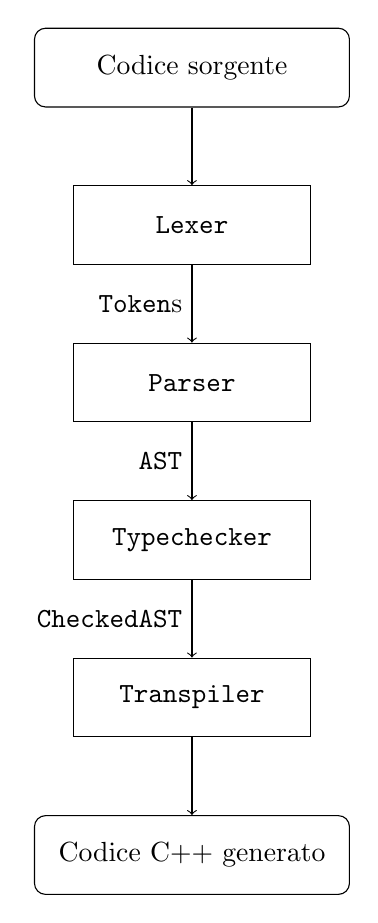
\begin{tikzpicture}[node distance=2cm]
		\node (source) [draw, rectangle, text centered, minimum width=4cm, minimum height=1cm, rounded corners] {Codice sorgente};
		\node (lexer) [below of=source, draw, rectangle, text centered, minimum width=3cm, minimum height=1cm] {\texttt{Lexer}};
		\node (parser) [below of=lexer, draw, rectangle, text centered, minimum width=3cm, minimum height=1cm] {\texttt{Parser}};
		\node (typechecker) [below of=parser, draw, rectangle, text centered, minimum width=3cm, minimum height=1cm] {\texttt{Typechecker}};
		\node (transpiler) [below of=typechecker, draw, rectangle, text centered, minimum width=3cm, minimum height=1cm] {\texttt{Transpiler}};
		\node (output) [below of=transpiler, draw, rectangle, text centered, minimum width=4cm, minimum height=1cm, rounded corners] {Codice C++ generato};

		\draw [->] (source) -- (lexer);
		\draw [->] (lexer) to node[left] {\texttt{Token}s} (parser);
		\draw [->] (parser) to node[left] {\texttt{AST}} (typechecker);
		\draw [->] (typechecker) to node[left] {\texttt{CheckedAST}} (transpiler);
		\draw [->] (transpiler) -- (output);
	\end{tikzpicture}}
	\caption{Moduli del processo di compilazione}
	\label{fig:moduli-compilatore}
\end{figure}

Nel seguente capitolo si descrive l'architettura del compilatore BugginOut, affrontando i moduli che lo compongono e le fasi del compilatore che realizzano. Nella figura sopra si pu\`o osservare l'architettura ad alto livello del compilatore che \`e costituito da quattro moduli principali:
\begin{itemize}
	\item \texttt{Lexer}: realizza l'analisi lessicale;
	\item \texttt{Parser}: realizza l'analisi sintattica;
	\item \texttt{Typechecker}: realizza l'analisi semantica;
	\item \texttt{Transpiler}: realizza la generazione del codice C++.
\end{itemize}
Questi interagiscono secondo un modello a \textit{pipeline}, in cui l'output di un modulo \`e l'input del successivo. Nel seguito si descriver\`a ciascuno di questi moduli e ci\`o che producono.

\section{\texttt{Lexer}}
\label{sec:lexer}

\begin{figure}[H]
	\centering
	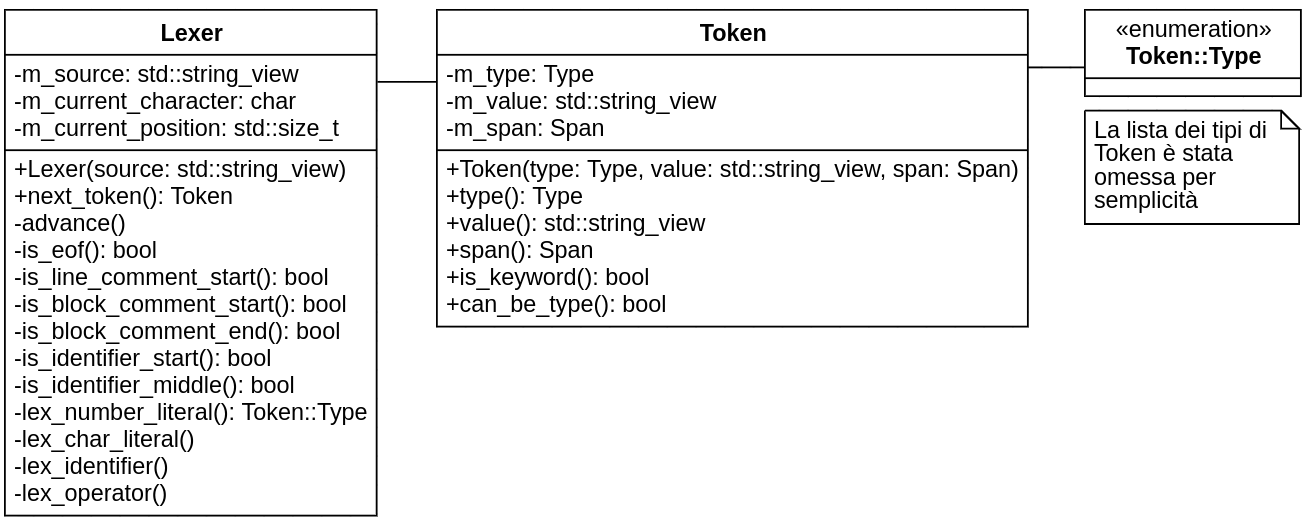
\includegraphics[width=0.9\textwidth]{figures/lexer.png}
	\caption{Diagramma UML del \texttt{Lexer}}
	\label{fig:lexer-uml}
\end{figure}

L'analisi lessicale \`e realizzata per mezzo di due classi: \texttt{Token} e \texttt{Lexer}.

La classe \texttt{Token} rappresenta i token generati dall'analisi lessicale ed \`e costituito da:
\begin{itemize}
	\item \texttt{type}: il tipo del token (un valore dell'enumerazione \texttt{Token::Type});
	\item \texttt{value}: il valore del token (una stringa);
	\item \texttt{span}: la posizione del token nel codice sorgente (un oggetto di tipo \texttt{Span}\footnote{Questo tipo di oggetto rappresenta una posizione all'interno del codice sorgente ed \`e non altro che un intervallo di due indici nella stringa contenente il sorgente del programma.}).
\end{itemize}

La classe \texttt{Lexer} realizza l'automa a stati finiti discusso nella sezione \ref{sec:analisi-lessicale} memorizzando:
\begin{itemize}
	\item \texttt{source}: il codice sorgente da analizzare (una stringa);
	\item \texttt{current\_character}: il carattere da analizzare (un carattere);
	\item \texttt{current\_position}: la posizione del prossimo carattere da analizzare (un intero).
\end{itemize}
Il metodo \texttt{advance} permette di avanzare l'automa al prossimo carattere, aggiornando \texttt{current\_character} e \texttt{current\_position} e, inoltre, di controllare se si \`e raggiunti la fine del codice sorgente. In tal caso, il metodo imposta \texttt{current\_character} al valore speciale $-1$.

Con il metodo \texttt{next\_token} \`e possibile avanzare l'automa e generare il prossimo token. Ogni volta che questo metodo viene chiamato si occuper\`a di:
\begin{itemize}
	\item rimuovere spazi vuoti e commenti;
	\item analizzare \texttt{current\_character} e generare il token corrispondente o generare un errore se il carattere non \`e valido.\footnote{Per la gestione degli errori si veda la sezione \ref{sec:gestione-degli-errori}}
\end{itemize}
In base al carattere incontrato, si delega il compito dell'analisi lessicale ad uno dei metodi presenti nel diagramma. Ad esempio, se il carattere incontrato \`e un numero si richiamer\`a il metodo \texttt{lex\_number\_literal}. Questo permette di mantenere il codice del \texttt{Lexer} pulito e facilmente estendibile, poich\'e ogni metodo si occupa di un caso specifico.

\section{\texttt{Parser}}
\label{sec:parser}

\begin{figure}[H]
	\centering
	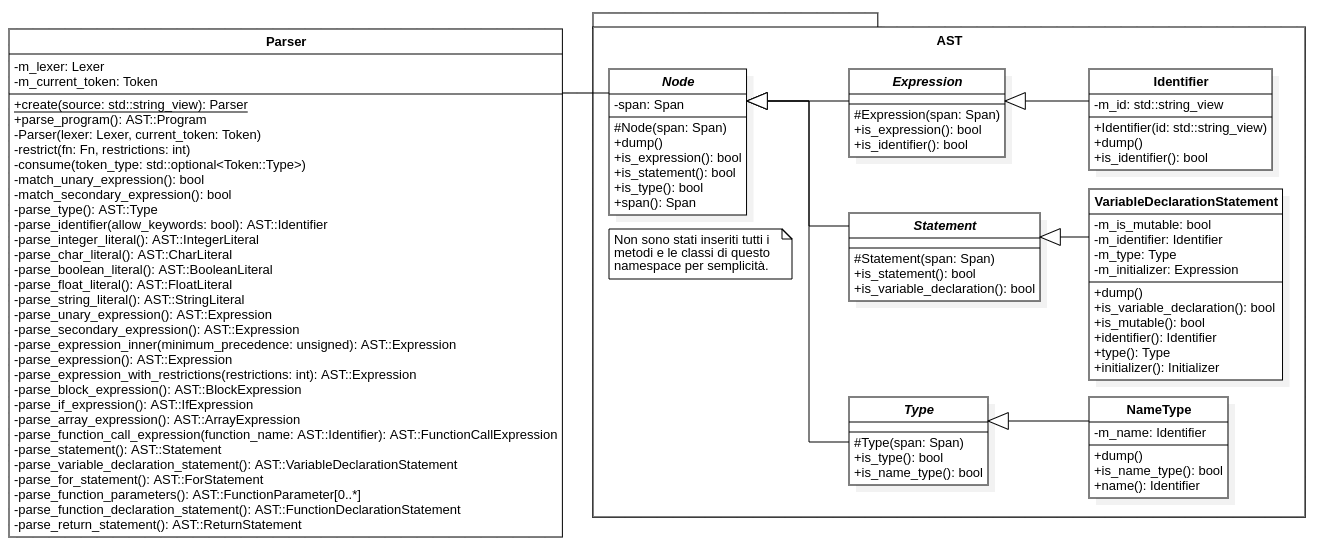
\includegraphics[width=0.9\textwidth]{figures/parser.png}
	\caption{Diagramma UML del \texttt{Parser}}
	\label{fig:parser-uml}
\end{figure}

L'analisi grammaticale \`e gestita dalla classe \texttt{Parser} che genera l'AST, rappresentato nell'omonimo \textit{namespace}, a partire dai token genrati dal \texttt{Lexer}.

Partiamo dal descrivere il \textit{namespace} \texttt{AST}. Questo contiene la classe madre \texttt{Node} che rappresenta un generico nodo dell'AST. L'unico suo attributo \`e \texttt{span}, la posizione nel codice sorgente. Da essa derivano le seguenti classi astratte:
\begin{itemize}
	\item \texttt{Expression}: rappresenta un'espressione, ovvero un nodo che restituisce un valore;
	\item \texttt{Statement}: rappresenta uno italiano, ovvero un nodo che non restituisce un valore;
	\item \texttt{Type}: rappresenta un tipo di dato.
\end{itemize}
Da ciascuna di queste a loro volta, derivano tutte le classi che rappresentano i nodi dell'AST. Ad esempio, come \`e possibile osservare nella figura \ref{fig:parser-uml}, possiamo osservare tre nodi:
\begin{itemize}
	\item \texttt{Identifier}: sottoclasse di \texttt{Expression}, rappresenta un identificatore ed \`e descritto dall'attributo stringa \texttt{id}.
	\item \texttt{VariableDeclarationStatement}: sottoclasse di \texttt{Statement}, rappresenta una dichiarazione di variable ed \`e descritto dagli attributi:
	\begin{itemize}
		\item \texttt{is\_mutable}: un booleano che indica se la variabile \`e mutabile o meno;
		\item \texttt{identifier}: il nome della variabile (un oggetto di tipo \linebreak \texttt{Identifier});
		\item \texttt{type}: il tipo della variabile (un oggetto di tipo \texttt{Type});
		\item \texttt{initializer}: l'inizializzatore della variabile (un oggetto di tipo \texttt{Expression}).
	\end{itemize}
	\item \texttt{NameType}: sottoclasse di \texttt{Type}, rappresenta un tipo di dato descritto da un singolo identificatore, il quale sar\`a un tipo primitivo (ad esempio: \texttt{i32} o \texttt{char}).
\end{itemize}

\`E bene notare che la classe \texttt{Node} definisce una serie di metodi importanti:
\begin{itemize}
	\item il metodo \texttt{dump} che permette di stampare in formato JSON l'intera struttura del nodo; questo risulta utile in fase di debugging per verificare l'AST generato dal \texttt{Parser}.
	\item i metodi \mbox{\texttt{is\_expression}, \texttt{is\_statement} e \texttt{is\_type}} che permettono di verificare il tipo di nodo; questi metodi sono utili per effettuare controlli e conversioni di tipo durante l'analisi semantica e la generazione del codice.
\end{itemize}

Come anticipato nella sezione \ref{sec:analisi-grammaticale}, la grammatica di questo linguaggio \`e LL(1) e, citando \cite{alfred2007compilers}:
\begin{parcolumns}[colwidths={1=0.44\textwidth,2=0.44\textwidth},rulebetween=true,nofirstindent=true,sloppy=true]{2}
	% LTeX: language=en_us
	\colchunk{
		\leftskip=1em
		``The first ``L'' in LL(1) stands for scanning the input from left to right, the second ``L'' for producing a leftmost derivation, and the ``1'' for using one input symbol of \emph{lookahead} at each step to make parsing action decisions.''
	}
	% LTeX: language=it
	\colchunk{
		\leftskip=1em
		``La prima ``L'' in LL(1) indica che si analizza l'input da sinistra verso destra, la seconda ``L'' indica che si produce una derivazione sinistra e l'``1'' per usare un \emph{lookahead} di un simbolo d'input a ogni passo per fare decisioni di analisi grammaticale.''
	}
	\colplacechunks
\end{parcolumns}

I parser costruiti per questo tipo di grammatica, e di conseguenza quella di BugginOut, sono detti \emph{predictive}, ovvero dei parser \emph{recursive descent} senza il bisogno di \emph{backtracking}. I parser \emph{recursive descent} sono dei particolari parser \emph{top-down} costruiti con delle procedure ricorsive dove ognuna di queste riflette un non-terminale della grammatica. Si \`e scelto di costruire il parser seguendo questo approccio proprio perch\'e il codice che ne risulta \`e molto semplice, leggibile ed efficiente, non essendo richiesto il backtracking. Di fatti, gli unici due attributi richiesti per mantenere lo stato del parser sono:
\begin{itemize}
	\item \texttt{lexer}: il \texttt{Lexer} che fornisce i token da analizzare;
	\item \texttt{current\_token}: il token corrente da analizzare.
\end{itemize}

Ogni metodo del parser, che rappresenta un non-terminale della grammatica, analizzer\`a il token corrente e, se corretto, lo \emph{consumer\`a}. Questa operazione viene implementata dal metodo \texttt{consume} e corrisponde ad ottenere il prossimo token dal \texttt{Lexer} e aggiornare \texttt{current\_token}. Il metodo prevede un parametro opzionale che permette di specificare il tipo di token atteso. Se il token corrente non corrisponde al tipo atteso, viene generato un errore di sintassi. Se il tipo di token non viene specificato, il metodo consuma il token corrente.

\`E importante notare che per realizzare dei \emph{predictive parser} la grammatica deve soddisfare due requisiti molto importanti:
\begin{itemize}
	\item non deve contenere ricorsioni sinistre;
	\item non deve essere ambigua.
\end{itemize}

La grammatica, per come \`e stata definita, non contiene ricorsioni sinistre ma \`e ambigua nella gestione delle espressioni e dei loro operatori. Questo \`e stato fatto volutamente per due ragioni:
\begin{itemize}
	\item \`e possibile cambiare la precedenza ed associativit\`a degli operatori in modo semplice, senza dover modificare la grammatica;
	\item il parser non spende tempo utile nell'analizzare produzioni \textit{singole} ovvero costituite da un solo non-terminale.
\end{itemize}
In ogni caso, l'amgiguit\`a deve essere gestita e, per farlo, si utilizza un algoritmo di \emph{precedence climbing}.

Introdotto per la prima volta da \cite{barron1981bcpl}, l'idea alla base \`e quella di avere una funzione ricevere in input un'espressione e una \emph{precedenza minima}. Durante l'analisi, la funzione consuma gli operandi fino a quando incontra operatori la cui precedenza \`e maggiore o uguale a quella minima. Se un operatore ha precedenza inferiore, l'espressione si interrompe e si ritorna al livello di ricorsione precedente. L'associativit\`a di un operatore viene gestita in maniera molto elegante, con un semplice controllo effettuato prima della prossima chiamata ricorsiva: se l'operatore \`e associativo a sinistra allora ne aumenta di un'unit\`a la precedenza, altrimenti la lascia invariata. Per capire meglio come funziona, vediamo degli esempi:
\begin{itemize}
	\item Si supponga di voler analizzare l'espressione \texttt{a + b + c}, che la precedenza di \texttt{+} sia 2 e che \texttt{+} sia associativo a sinistra.

	La prima chiamata ricorsiva consuma \texttt{a} e chiama la funzione con precedenza minima $2 + 1$ essendo \texttt{+} associativo a sinistra. La prossima chiamata trover\`a nuovamente \texttt{+} con precedenza $2$ minore della precedenza minima $2 + 1$. Allora esce e l'espressione generata sar\`a \linebreak \texttt{(a + b) + c}.
	\item Adesso si supponga di essere nelle stesse condizioni dell'esempio precedente con l'unica differenza che \texttt{+} sia associativo a destra.

	Durante l'analisi la seconda chiamata alla funzione avr\`a precedenza minima $2$ e, dunque, quando incontrer\`a \texttt{+} lo consumer\`a e l'espressione generata sar\`a \texttt{a + (b + c)}.
\end{itemize}

Questo algoritmo \`e implementato tramite tre funzioni:
\begin{itemize}
	\item \texttt{parse\_expression\_inner}: \`e la funzione ricorsiva di cui si \`e discusso fino ad ora;
	\item \texttt{parse\_primary\_expression}: \`e la funzione che analizza il non-terminale \texttt{<primary>};
	\item \texttt{parse\_secondary\_expression}: \`e la funzione che, prese la parte sinistra e l'operatore di un'espressione ottenuti da \linebreak \texttt{parse\_expression\_inner}, analizza la parte destra (se necessario) e li combina per ottenere l'espressione intermedia.
\end{itemize}
Per gestire la precedenza e l'associativit\`a degli operatori si usa una classe ausiliaria detta \texttt{OperatorData} che mantiene questi due valori per ognuno degli operatori. Per rappresentare la precedenza si usa un intero senza segno che, se basso indica una bassa precedenza, se alto indica una alta precedenza. Per l'associativit\`a si usa una semplice enumerazione di due valori: \texttt{Left} se a sinistra e \texttt{Right} se a destra.

\section{\texttt{Typechecker}}
\label{sec:typechecker}

L'analisi semantica \`e realizzata con la classe \texttt{Typechecker} che si occupa di arrichire l'AST, generando il \texttt{CheckedAST}, con le informazioni di tipo rappresentate nel \textit{namespace} \texttt{Types}.

\begin{figure}[H]
	\centering
	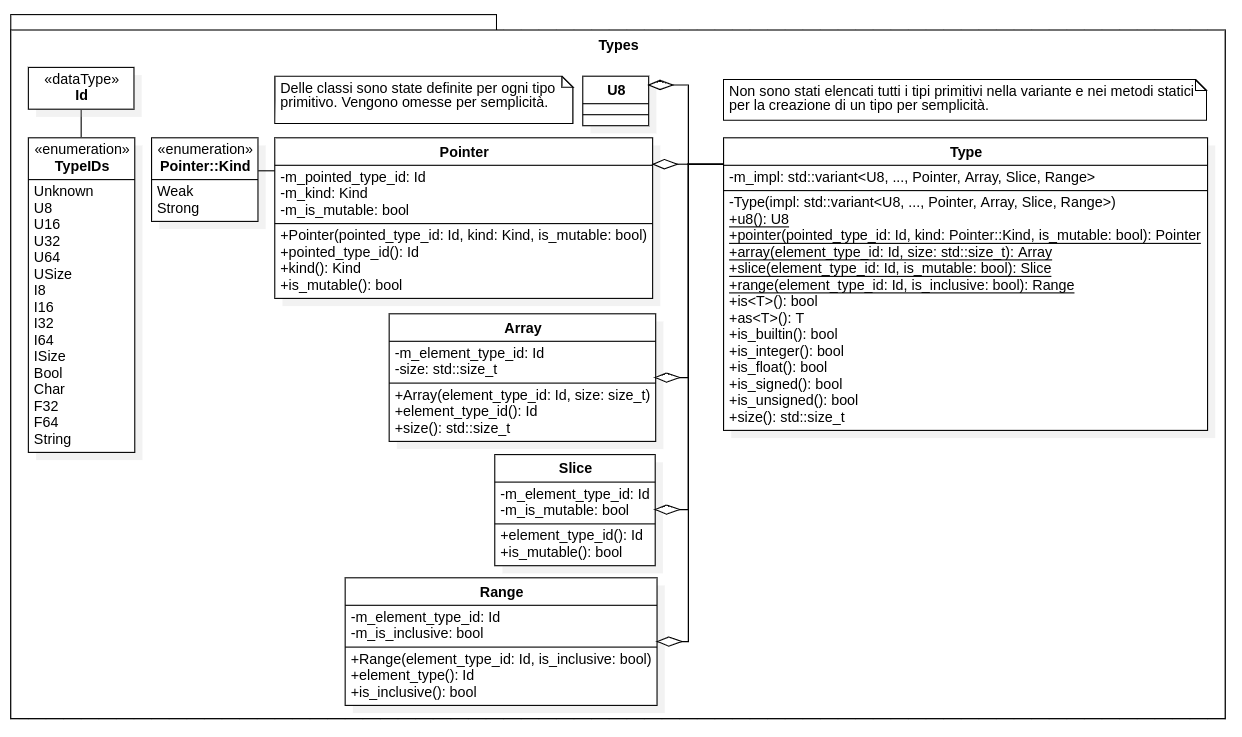
\includegraphics[width=0.9\textwidth]{figures/types.png}
	\caption{Diagramma UML del \textit{namespace} \texttt{Types}}
	\label{fig:typechecker-types}
\end{figure}

Il \textit{namespace} \texttt{Types} si occupa del \emph{type system} e contiene:
\begin{itemize}
	\item delle classi vuote per ogni tipo primitivo (\texttt{U8}, \texttt{U16}, ...);
	\item le classi \texttt{Pointer}, \texttt{Array}, \texttt{Slice} e \texttt{Range} per i rispettivi tipi;
	\item la classe \texttt{Type}.
\end{itemize}
Le classi per i tipi composti contengono ciasuna le propriet\`a relative al tipo rappresentato. Ad esempio, la classe \texttt{Array} memorizza la dimensione e il tipo degli elementi, mentre \texttt{Range} memorizza il tipo dell'intervallo e se l'estremo superiore \`e incluso.

La classe \texttt{Type} funge da \textit{wrapper} attorno ad un \textit{sum-type} che rappresenta un'unione disgiunta di tutte le classi viste sopra. L'adozione di un \textit{sum-type}, anzich\'e di una gerarchia di classi, consente una maggiore \textit{type safety} e una rappresentazione pi\`u efficiente senza allocazioni sull'\textit{heap}.

La clase \texttt{Type} definisce dei metodi per creare dei tipi specifici (ad esempio, \texttt{u8}, \texttt{pointer}, \texttt{array}, ...), nonch\'e dei metodi di introspezione (ad esempio, \texttt{is}, \texttt{is\_integer}, \texttt{size}, ...) utili per verificare la propriet\`a di un tipo. Infine, fornisce il metodo \texttt{as} per accedere direttamente alla rappresentazione concreta del tipo.

\begin{figure}[H]
	\centering
	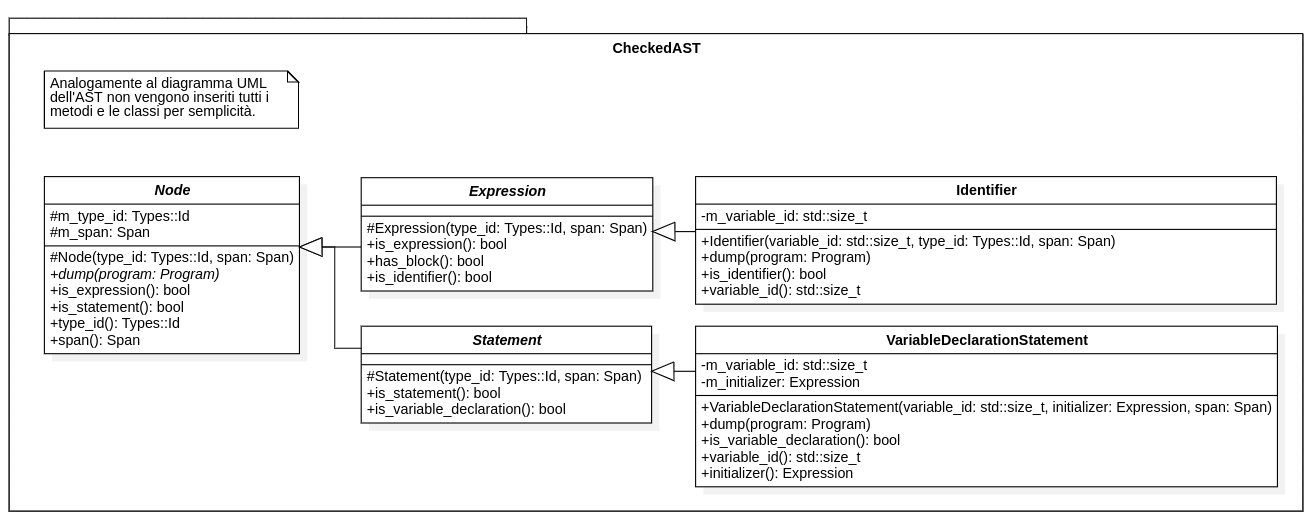
\includegraphics[width=0.9\textwidth]{figures/checked_ast.png}
	\caption{Diagramma UML del \textit{namespace} \texttt{CheckedAST}}
	\label{fig:checked-ast-uml}
\end{figure}

Il \texttt{CheckedAST} \`e una struttura analoga all'\texttt{AST} originale, ma arricchita con informazioni di tipo. L'arricchimento consiste nell'aggiunta, in ciascun \texttt{Node}, di un attributo \texttt{type} di tipo \texttt{Types::Id}. Quest'ultimo rappresenta un identificatore numerico univoco del tipo, il cui significato sarà chiarito nel paragrafo dedicato alla classe \texttt{Typechecker}. Una differenza sostanziale rispetto all'\texttt{AST} è la rimozione del sottoalbero di classi \texttt{Type}, le cui informazioni vengono ora riassunte tramite l'identificatore del tipo.

\begin{figure}[H]
	\centering
	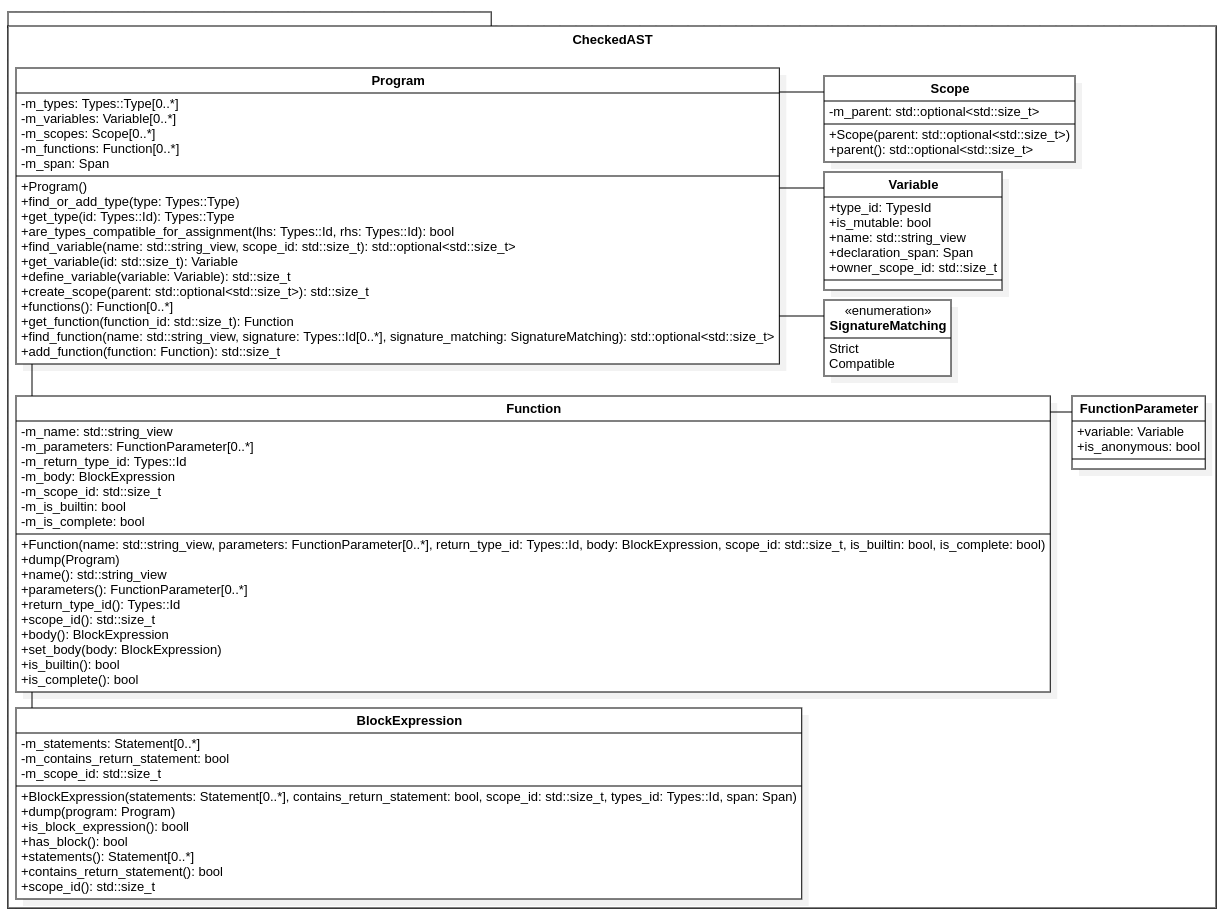
\includegraphics[width=0.9\textwidth]{figures/checked_ast_program.png}
	\caption{Diagramma UML della classe \texttt{CheckedAST::Program}}
	\label{fig:checked-ast-program-uml}
\end{figure}

All'interno del \texttt{CheckedAST} viene definita la classe \texttt{Program}. Questa \`e particolarmente importante in quanto contiene una serie di attributi che cade sotto il termine ombrello di \emph{tabella dei simboli}:
\begin{itemize}
	\item \texttt{scopes}: \`e una lista di oggetti di tipo \texttt{Scope} che rappresentano gli \emph{scope} (ambito di visibilit\`a) del programma, ovvero la porzione di codice in cui una variabile \`e visibile e utilizzabile; ognuno di questi contiene un riferimento opzionale allo \textit{scope} genitore.
	\item \texttt{functions}: \`e una lista di oggetti di tipo \texttt{Function} che contiene tutte le funzioni dichiarate nel programma, costituite da:
	\begin{itemize}
		\item \texttt{name}: il nome della funzione;
		\item \texttt{parameters}: una lista di oggetti di tipo \texttt{FunctionParameter} che rappresentano i parametri della funzione, ognuno dei quali contiene un oggetto di tipo \texttt{Variable} che rappresenta la sua dichiarazione e un booleano che indica se \`e \emph{anonimo};
		\item \texttt{return\_type}: l'identificatore del tipo di ritorno della funzione;
		\item \texttt{body}: il corpo della funzione, un oggetto di tipo \texttt{BlockExpression};
		\item \texttt{scope\_id}: l'identificatore dello \textit{scope} dei parametri della funzione.
		\item \texttt{is\_builtin}: un booleano che indica se \`e una funzione predefinita del linguaggio;
		\item \texttt{is\_complete}: un booleano che indica se la funzione \`e completa o meno; una funzione \`e considerata completa se il suo corpo \`e stato analizzato.
	\end{itemize}
	\item \texttt{variables}: è una lista di oggetti di tipo \texttt{Variable} che contengono informazioni sulle variabili dichiarate nel programma e sono:
	\begin{itemize}
		\item \texttt{type\_id}: l'ID del tipo della variabile;
		\item \texttt{is\_mutable}: un booleano che indica se la variabile \`e mutabile o meno;
		\item \texttt{name}: il nome della variabile;
		\item \texttt{declaration\_span}: la posizione della dichiarazione della variabile;
		\item \texttt{owner\_scope\_id}: l'ID dello \emph{scope} della variabile.
	\end{itemize}
\end{itemize}

\begin{figure}[H]
	\centering
	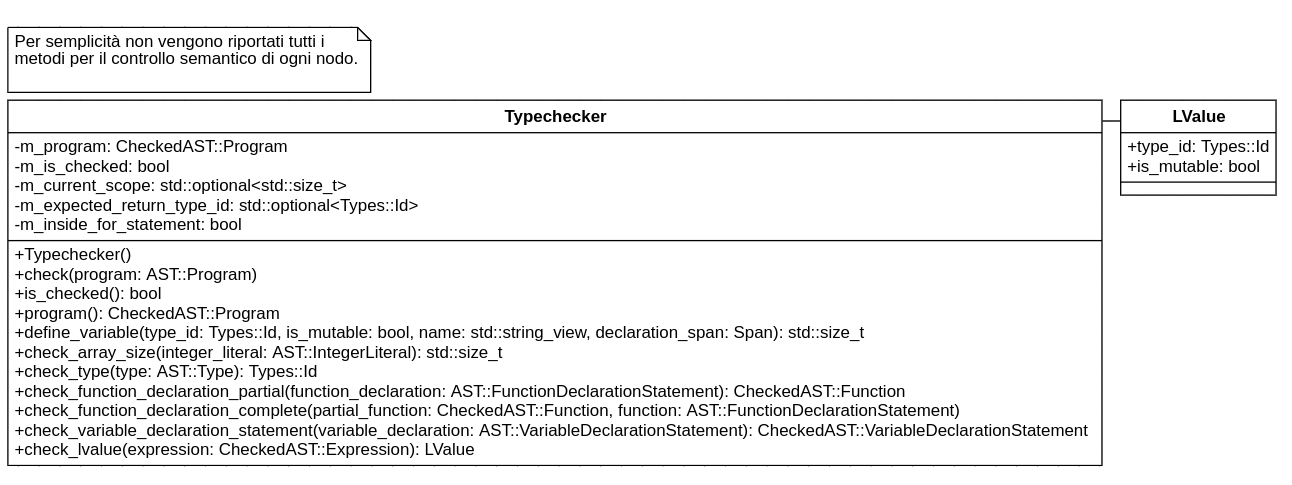
\includegraphics[width=0.9\textwidth]{figures/typechecker.png}
	\caption{Diagramma UML della classe \texttt{Typechecker}}
	\label{fig:typechecker-uml}
\end{figure}

Una volta delineate le basi strutturali del \texttt{Typechecker}, si pu\`o passare a descrivere il suo compito e funzionamento. Oltre che di costruirlo, si occupa di fare i controlli semantici sul programma. L'approccio utilizzato \`e il \emph{bidirectional typechecking}, introdotto da \cite{pierce2000local}.
\begin{parcolumns}[colwidths={1=0.44\textwidth,2=0.44\textwidth},rulebetween=true,nofirstindent=true,sloppy=true]{2}
	% LTeX: language=en_us
	\colchunk{
		\leftskip=1em
		``[\dots] the typechecker operates two distinct modes: \emph{synthesis} mode, where typing information is propagated upward from subexpressions, and \emph{checking} mode, where information is propagated downward from enclosing expressions. Synthesis mode [\dots] is used when we do not know anything about the expected type of an expression [\dots]. Checking mode is used when the surrounding context determines the type of the expression and we only need to check that it does have that type.''
	}
	% LTeX: language=it
	\colchunk{
		\leftskip=1em
		``[\dots] il typechecker opera in due modalit\`a distinte: la modalit\`a di \emph{sintesi}, dove le informazioni di tipo vengono propagate verso l'alto dalle sottoespressioni, e la modalit\`a di \emph{controllo}, dove le informazioni vengono propagate verso il basso dalle espressioni pi\`u esterne. La modalit\`a di sintesi [\dots] \`e usata quando non sappiamo nulla sul tipo atteso di un'espressione [\dots]. La modalit\`a di controllo \`e usata quando il contesto circostante determina il tipo dell'espressione e bisogna solo controllare che abbia quel tipo.''
	}
	\colplacechunks
\end{parcolumns}

In seguito ci riferiremo alla modalit\`a di controllo con \emph{check} e a quella di sintesi con \emph{infer}, per riflettere meglio la terminologia usata nel \texttt{Typechecker}.

Ogni nodo del \texttt{CheckedAST} viene verificato tramite un metodo \texttt{check} apposito che si occupa di verificarne la correttezza semantica, richiamando ricorsivamente i metodi \texttt{check} per ogni nodo figlio fino a quando non si raggiungono le foglie. Eseguiti tutti i controlli semantici, se questi hanno avuto successo, il metodo restituisce il nodo corrispondente del \texttt{CheckedAST}, altrimenti si genera un errore semantico.

Attualmente, il \texttt{Typechecker} effettua una sola operazione di tipo \textit{infer}. Questa si trova nella gestione delle dichiarazioni delle variabili con tipo implicito. In questo caso, si analizzer\`a l'inizializzatore della variabile con una chiamata a \texttt{check\_expression} e, in caso di successo, si otterr\`a il tipo dell'espressione. Questo tipo viene dunque utilizzato come tipo della variabile dichiarata.\footnote{Sull'inferenza, e come questa pu\`o essere utilizata nel futuro del linguaggio, si discuter\`a nelle conclusioni.}

\begin{figure}[H]
	\centering
	\begin{minted}[breaklines,frame=lines,fontsize=\footnotesize]{text}
fn foo(): i32 { 42 }

fn main(): void {
    var a = foo();
}
  \end{minted}
	\caption{Esempio d'inferenza del tipo di una variabile}
	\label{fig:typechecker-var-decl-infer}
\end{figure}

Nel codice riportato qui sopra la variabile \texttt{a} viene dichiarata senza un tipo esplicito, dunque il \texttt{Typechecker} deve analizzare l'espressione inizializzata. Analizzandola, trova una chiamata di funzione; la funzione richiamata è \texttt{foo}, le cui informazioni sono reperibili nella lista functions del programma. Trovata la funzione, si osserva che il suo tipo di ritorno è \texttt{i32}. È possibile dunque concludere che il tipo della chiamata di funzione sarà lo stesso e, di conseguenza, anche quello della variabile.

\section{\texttt{Transpiler}}
\label{sec:transpiler}

\section{Gestione degli errori}
\label{sec:gestione-degli-errori}
